\documentclass{article}

\usepackage {titlesec}
\usepackage[utf8]{inputenc}
\usepackage[english,russian]{babel}

% Offset setup %
\usepackage[left=15mm,
            top=15mm, 
            right=10mm,
            bottom=15mm, nohead, nofoot]{geometry}

% Maths packages %
\usepackage{amssymb}
\usepackage{amsmath}

% Special symbols %
\usepackage{wasysym}
\usepackage{cancel}
\usepackage{graphicx}
\usepackage{numprint}
\graphicspath{{pictures/}}

\titlespacing*{\section}{\parindent}{*4}{*4}



\title{Домашнее задание 18}
\author{Ткачев Андрей, группа 166}
\date{\today}

% Other%
\newcommand{\pr}{^{\prime}}
\newcommand{\ppr}{^{\prime\prime}}
\newcommand{\xp}{x^{\prime}}
\newcommand{\xpp}{x^{\prime\prime}}
\newcommand{\xppp}{x^{\prime\prime\prime}}
% Alias %
\newcommand{\pair}[2]{(#1,\ #2)}
\newcommand{\andi}{$ и $}
\newcommand{\xor}{\oplus}
%\newcommand{\xor}{\oplus}%

% Fracs %
\newcommand{\half}[1]{\frac{#1}{2}}
% Pretty Num letters%
\newcommand{\N}{\mathbb{N}}
\newcommand{\R}{\mathbb{R}}
\newcommand{\Q}{\mathbb{Q}}
\newcommand{\M}{\mathbb{M}}
\newcommand{\conti}{2^{\N}}

% Vector graphics %
\usepackage{tikz}
\definecolor{white}{rgb}{1.0, 1.0, 1.0}
\definecolor{black}{rgb}{0.0, 0.0, 0.0}
\definecolor{royalblue}{RGB}{255,170,128}
\definecolor{lgr}{RGB}{168, 228, 160}
\definecolor{lblue}{RGB}{24,205,255}

\usetikzlibrary{decorations.markings}
\usetikzlibrary{shapes.geometric}

\pgfdeclarelayer{edgelayer}
\pgfdeclarelayer{nodelayer}
\pgfsetlayers{edgelayer,nodelayer,main}

\tikzstyle{none}=[inner sep=0pt]
\tikzstyle{node}=[circle,fill=white,draw=black,thick]

\begin{document}
    \maketitle
    \paragraph{Задача 1.} Приведем в качестве доказательства схему вычисляющую $XOR(x, y, z)$. 
    \begin{center}
        \begin{tikzpicture}
            \begin{pgfonlayer}{nodelayer}
            \node [style = node] (x) at (-4, 0) {$x$};
            \node [style = node] (y) at (-2, 0) {$y$};
            \node [style = node] (z) at (0, 0) {$z$};

            \node [style = node] (and1) at (-6, -1.5) {$\wedge$};
            \node [style = node] (and2) at (-4, -1.5) {$\wedge$};
            \node [style = node] (and3) at (-2, -1.5) {$\wedge$};

            \node [style = node] (or_0) at (1, -1) {$\vee$};
            \node [style = node] (or_1) at (1, -2) {$\vee$};

            \node [style = node] (and) at (-2, -3) {$\wedge$};
            \node [style = node] (or1) at (-6, -3) {$\vee$};
            \node [style = node] (and4) at (-2, -3) {$\wedge$};
            
            \node [style = node] (or3) at (-6, -4.5) {$\vee$};

            \node [style = node] (notn) at (-6, -6) {$\lnot$};s
            \node [style = node] (and5) at (-2, -6) {$\wedge$};

            \node [style = node, fill=royalblue] (or5) at (0, -6) {$\lor$};
            \end{pgfonlayer}

        \begin{pgfonlayer}{edgelayer}
            \draw [->, thick] (x) to (and1);
            \draw [->, thick] (x) to (and2);
            \draw [->, thick] (x) to (or_1);

            \draw [->, thick] (y) to (and1);
            \draw [->, thick] (y) to (and3);
            \draw [->, thick] (y) to (or_0);
 
            \draw [->, thick] (z) to (and2);
            \draw [->, thick] (z) to (and3);
            \draw [->, thick] (z) to (or_0);

            \draw [->, thick] (or_0) to (or_1);
            \draw [->, thick] (or_1) to (and5);
            \draw [->, thick] (and1) to (or1);
            \draw [->, thick] (and2) to (or1);
            \draw [->, thick] (and3) to (or3);
            \draw [->, thick] (or1) to (or3);


            \draw [->, thick] (and2) to (and);
            \draw [->, thick] (and3) to (and);

            \draw [->, thick] (and) to (or5);            

            \draw [->, thick] (or3) to (notn);
            \draw [->, thick] (notn) to (and5);
            \draw [->, thick] (and5) to (or5);
        \end{pgfonlayer}
    \end{tikzpicture}
    \end{center}
    $x \oplus y \oplus z$ принимает значение 0 либо когда $x=y=z=0$, либо когда какие-то 2 переменные равны 1, а третья --- 0; в остальных случаях (только один истинный аргумент или все аргументы истинны) значение --- 1.  Сообственно, приведенная схема ведет себя так же.

    \paragraph{Задача 2.}
    Последние 9 наборов значений переменных $x_1, x_2, x_3, x_4$ в стандартном порядке имеют вид
    \begin{itemize}
        \item 0111
        \item 1000
        \item 1001
        \vdots
        \item 1111
    \end{itemize}

    Эти наборы отличаются от оставшихся тем, что в них старший бит равен 1 или последние три бита равны 1. В виде схемы последнее предложение записывается так:

    \begin{center}
    \begin{tikzpicture}
        \begin{pgfonlayer}{nodelayer}
            \node [style = node] (x1) at (-6, 0) {$x_1$};
            \node [style = node] (x2) at (-4, 0) {$x_2$};
            \node [style = node] (x3) at (-2, 0) {$x_3$};
            \node [style = node] (x4) at (0, 0) {$x_4$};
            \node [style = node] (and1) at (-2, -1.5) {$\wedge$};
            \node [style = node] (and2) at (-4, -3) {$\wedge$};
            \node [style = node, fill=royalblue] (or) at (-6, -4.5) {$\wedge$};
        \end{pgfonlayer}

        \begin{pgfonlayer}{edgelayer}
            \draw [->, thick] (x3) to (and1);
            \draw [->, thick] (x4) to (and1);
            \draw [->, thick] (x2) to (and2);
            \draw [->, thick] (and1) to (and2);
            \draw [->, thick] (and2) to (or);
            \draw [->, thick] (x1) to (or);
        \end{pgfonlayer}
    \end{tikzpicture}
    \end{center}

    Длина данной схемы равна 7, что явно меньше 15, и она вычисляет требуемую функцию.

    \paragraph{Задача 3.}
    Обозначим за элемент $P$ с тремя входами и одним выходом следущую схему:

    \begin{center}
    \begin{tikzpicture}
        \begin{pgfonlayer}{nodelayer}
            \node [style = node] (x1) at (-4, 0) {$x_1$};
            \node [style = node] (x2) at (-2, 0) {$x_2$};
            \node [style = node] (x3) at (0, 0) {$x_3$};
            \node [style = node] (and1) at (-4, -1.5) {$\wedge$};
            \node [style = node, fill=royalblue] (and2) at (-4, -3) {$\wedge$};
            \node [style = node] (not) at (-2, -1.5) {$\lnot$};
        \end{pgfonlayer}

        \begin{pgfonlayer}{edgelayer}
            \draw [->, thick] (x1) to (and1);
            \draw [->, thick] (x3) to (and1);
            \draw [->, thick] (x2) to (not);
            \draw [->, thick] (and1) to (and2);
            \draw [->, thick] (not) to (and2);
        \end{pgfonlayer}
    \end{tikzpicture}
    \end{center}

    Нетрудно видеть, что данная схема вычисляет функцию, которая истинна только на наборе аргументов $1, 0, 1$ (порядок важен). Тогда составим схему для входа размера $n$, определяющую, входит ли подстрока $101$ в $x_1x_2 \ldots x_n$..

    \begin{center}
    \begin{tikzpicture}
        \begin{pgfonlayer}{nodelayer}
            \node [style = node] (x1) at (-10, 0) {$x_1$};
            \node [style = node] (x2) at (-8, 0) {$x_2$};
            \node [style = node] (x3) at (-6, 0) {$x_3$};
            \node [] (ldots) at (-4, 0) {$\ldots\ldots$};
            \node [style = node] (xn2) at (-2, 0) {$x_{n-2}$};
            \node [style = node] (xn1) at (0, 0) {$x_{n-1}$};
            \node [style = node] (xn) at (2, 0) {$x_{n}$};

            \node [style = node] (p1) at (-10, -1.5) {$P$};
            \node [style = node] (p2) at (-8, -1.5) {$P$};
            \node [] (p_fake) at (-6, -1.5) {$\ldots\ldots$};
            \node [style = node] (pn) at (-2, -1.5) {$P$};

            \node [style = node] (or1) at (-10, -3) {$\vee$};
            \node [style = node] (or2) at (-10, -4.5) {$\vee$};
            \node [] (vdots) at (-10, -6) {$\vdots$};
            \node [style = node, fill=royalblue] (orn) at (-10, -7.5) {$\vee$};
        \end{pgfonlayer}

        \begin{pgfonlayer}{edgelayer}
            \draw [->, thick] (x1) to (p1);
            \draw [->, thick] (x2) to (p1);
            \draw [->, thick] (x3) to (p1);
            
            \draw [->, thick] (x2) to (p2);
            \draw [->, thick] (x3) to (p2);
            \draw [->, thick, dotted] (ldots) to (p2);

            \draw [->, thick] (xn2) to (pn);
            \draw [->, thick] (xn1) to (pn);
            \draw [->, thick] (xn) to (pn);

            \draw [->, thick] (p1) to (or1);
            \draw [->, thick] (p2) to (or1);

            \draw [->, thick] (or1) to (or2);
            \draw [->, thick, dotted] (p_fake) to (or2);
            \draw [->, thick] (pn) to (orn);

        \end{pgfonlayer}
    \end{tikzpicture}
    \end{center}

    Корректность работы схемы можно доказать по индукции по размеру входа (База: $n = 3$, результатом является просто результат работы схемы $P$, которая корректна. Предположение: верно для $n=k$. Шаг: строка из $k + 1$ аргументов содержит подстроку $101$ если ее содержит подстрока из первых $k$ аргументов или последние три аргумета, т.е. результат работы схемы на этом входе --- дизъюнкиция выхода схемы на $k$ аргументов и схемы $P$ на последних трех аргументах, что и требовалось).

    Оценим размер полученной схемы. Зная, что $|P| = 3$, получаем, что размер схемы 
    $$n + \underbrace{(n - 2)|P|}_{\text{n - 2 раза используем схему $P$}} + \underbrace{(n - 3)}_{\text{n - 3 раза используем дизъюнкцию}} = $$
    $$=  n + 3n - 6 + n - 3 = 5n - 9 = O(n)$$

    \paragraph{Задача 4.}
    Умножение двоичного числа на 3 равносильно сумме этого числа и его же, умноженного на 2.

    Умножение двоичного числа на 2 есть приписывание к нему справа нулевого бита.

    Если двоичное число в своей записи имеет $n$ бит, то результатом умножения на три можест стать $n + 2$ битное число. Таким образом, мы строим схему на $n$ входов $x_n, \ldots, x_1$ (пусть $x_n$ - страший бит) и $n + 2$ выходами $y_{n+2}, \ldots, y_{1} $.

    Суммирование реализуем, как обычное сложение столбиком
    \begin{center}
    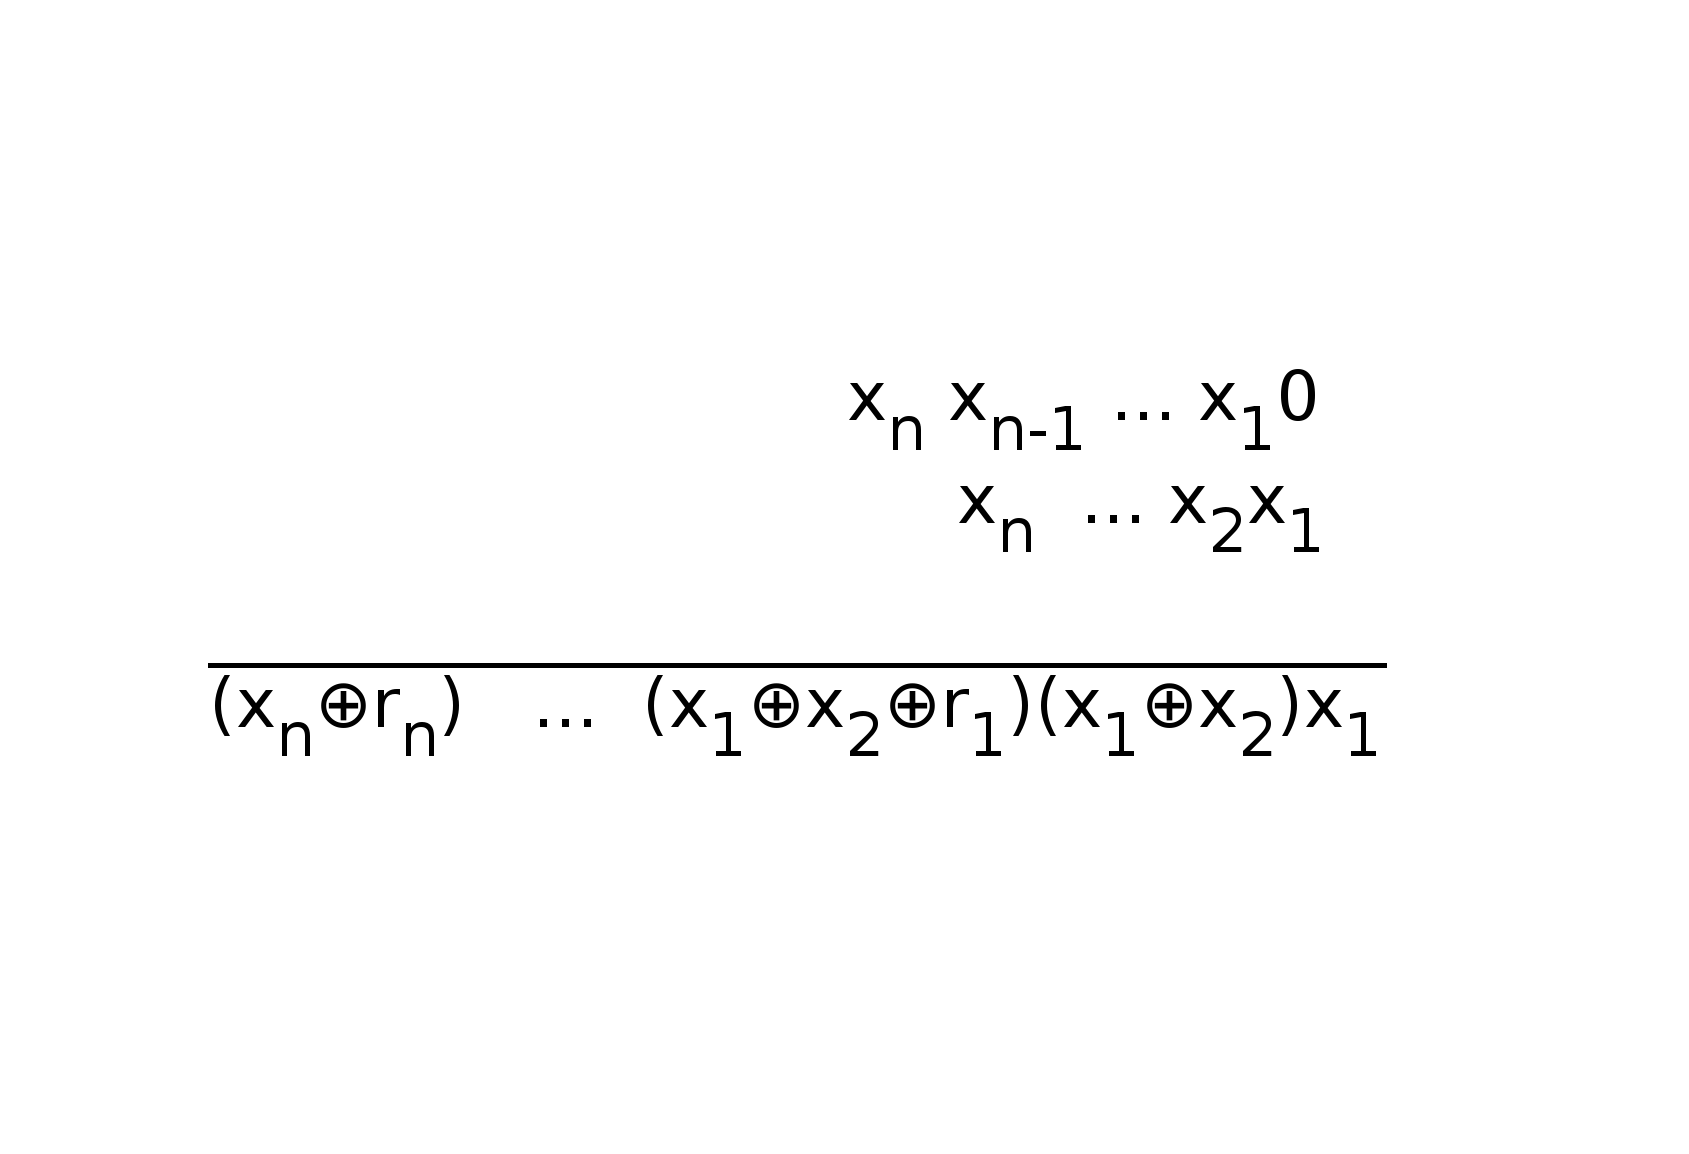
\includegraphics[scale=0.7]{aaaa}
    \end{center}

    Для красоты введем вспомогательную схему $S$ с тремя входами --- аргументы сложения и значение, которое переносится с прошлых разрядов, и двумя выходами --- результат сложения по модулю и число, которое необходимо перенести в следущий разряд (1, если единиц среди аргументов больше одной).

    \begin{center}
    \begin{tikzpicture}
        \begin{pgfonlayer}{nodelayer}
            \node [style = node] (x1) at (-4, 0) {$x_1$};
            \node [style = node] (x2) at (-2, 0) {$x_2$};
            \node [style = node] (r) at (0, 0) {$x_3$};
            \node [style = node] (xor1) at (0, -1.5) {$\oplus$};
            \node [style = node, fill=lgr] (xor2) at (-2, -3) {$\oplus$};
            \node [style = node, fill=lblue] (maj) at (-4, -3) {$Maj_3$};
        \end{pgfonlayer}

        \begin{pgfonlayer}{edgelayer}
            \draw [->, thick] (r) to (xor1);
            \draw [->, thick] (x1) to (xor2);
            \draw [->, thick] (xor1) to (xor2);
            \draw [->, thick] (x2) to (xor1);
            \draw [->, thick] (x1) to (maj);
            \draw [->, thick] (x2) to (maj);
            \draw [->, thick] (r) to (maj);
        \end{pgfonlayer}
    \end{tikzpicture}
    \end{center}
    
    Зеленый выход --- результат сложения, который будет записан в разряд, синий --- число для переноа в следующий разряд.

    Позволим себе использовать элемент <<$0$>> (т.к. мы его можем получить из $x \wedge \bar{x}$). Будем считать так же, что если на изображение в $S$ входит только две <<стрелки>> причем одна из них от нуля, то это означает, что недостающие аргументы --- нули (во избежание нагромаждения стрелок).

    \begin{center}
    \begin{tikzpicture}
        \begin{pgfonlayer}{nodelayer}
            \node [style = node] (zero2) at (-10, 0) {$0$};
            \node [style = node] (xn) at (-8, 0) {$x_{n}$};
            \node [style = node] (xn1) at (-6, 0) {$x_{n-1}$};
            \node [] (ldots) at (-4, 0) {$\ldots\ldots$};
            \node [style = node] (x2) at (-2, 0) {$x_2$};
            \node [style = node] (x1) at (0, 0) {$x_1$};

            \node [style = node] (not) at (2, 0) {$\lnot$};
            \node [style = node] (zero) at (2, -1.5) {$\wedge$};            

            \node [style = node] (sn1) at (-8, -3) {$S$};
            \node [style = node] (sn) at (-6, -3) {$S$};
            \node [] (ldots2) at (-4, -3) {$\ldots\ldots$};
            \node [style = node] (s2) at (0, -3) {$S$};
            \node [style = node] (s1) at (2, -3) {$S$};

            \node [style = node, fill=royalblue] (an2)  at (-10, -4.5) {$a_{n+2}$};
            \node [style = node, fill=royalblue] (an1) at (-8, -4.5) {$a_{n+1}$};
            \node [style = node, fill=royalblue] (an) at (-6, -4.5) {$a_n$};
            \node [] (ldots3) at (-4, -4.5) {$\ldots\ldots$};
            \node [style = node, fill=royalblue] (a2) at (0, -4.5) {$a_2$};
            \node [style = node, fill=royalblue] (a1) at (2, -4.5) {$a_1$};
        \end{pgfonlayer}

        \begin{pgfonlayer}{edgelayer}
            \draw [green, ->, semithick] (s1) to (a1);
            \draw [green, ->, semithick] (s2) to (a2);
            \draw [green, ->, semithick] (sn) to (an);
            \draw [green, ->, semithick] (sn1) to (an1);

            \draw [blue, ->, thick] (s1) to (s2);
            \draw [blue, ->, thick, dotted] (s2) to (-2, -3);
            \draw [blue, ->, thick] (sn) to (sn1);
            \draw [blue, ->, thick] (sn1) to (an2);

            \draw [->, thick] (x1) to (s1);
            \draw [->, thick] (x1) to (not);
            \draw [->, thick] (not) to (zero);
            \draw [->, thick] (zero) to (s1);

            \draw [->, thick] (x1) to (s2);
            \draw [->, thick] (x2) to (s2);
            \draw [->, thick] (xn1) to (sn);
            \draw [->, thick] (xn) to (sn);

            \draw [->, thick] (xn) to (sn1);
            \draw [->, thick] (zero2) to (sn1);
        \end{pgfonlayer}
    \end{tikzpicture}
    \end{center}

    Оценим размер схемы $S$. В ней используется два $xor$, каждый из которых требует 5 базисных функций (два отрицания, две конъюнкции и дизъюнкция) и функция $Maj_3$, которая записывается за 4 базовых функции (две конъюнкции и две дизъюнкции). Итого: $|S| = 14$.

    Теперь оценим нашу схему. В ней используется ровно $n + 1$ подсхема $S$, две элементарных функции для получения нуля и $n$ аргументнов. Итого: $(n + 1) |S| + n + 2 =14n + 16= O(n)$.

    \paragraph{Задача 5.}
    Воспользуемся признаком делимости на 3 в четверичной системе счисления: число делится на 3 в четверичной системе счисления, когда его сумма цифр делится на 3 (следует из того, что в этой системе $i$-ый разряд на самом деле является числом $4^i \cdot a = (4^i - 1)a + a = (4 - 1)(\ldots)a + a = 3(...)a + a$, т.е. любое число можно записать как сумму цифр и некую сумму чисел, кратных трем). Из четверичной системы мы можем легко перейти в двоичную --- достаточно каждую цифру представить как двочиное двухбитное число. Тогда получим признак делимости на 3 для двоичных чисел: двоичное число делится на три, если сумма чисел, образованных битами $0$ и $1$, $2 \andi 3 \ldots, n - 1\andi n$ делится на три.

    Реализуем схему $P$, которая будет однократно выполнять суммирование, описанное выше, чтобы после многократноего ее применения получиль простое двухбитное число, для которого понятно, как определить кратность.

    Для начала при помощи схемы суммирования бит $S$ из одной из прошлых задач построим схему сумматора $\sum$ с $2n$ входами и $n$ выходами (т.е. в результате указанного суммирования мы не можем получить число больше исходного(так если мы выполним суммировние для $2^{n + 1} - 1$ мы получим число не больше, чем $\half{3n}$, двоичная запись которого много меньше $n$ бит).

    \begin{center}
    \begin{tikzpicture}
        \begin{pgfonlayer}{nodelayer}
            \node [style = node] (not) at (0, 0) {$\lnot$};
            \node [style = node] (zero) at (0, -1.5) {$\wedge$}; 

            \node [style = node] (yn) at (-6, 0) {$y_{n}$};
            \node [] (ldots2) at (-4, 0) {$\ldots\ldots$};
            \node [style = node] (y1) at (-2, 0) {$y_1$};

            \node [style = node] (xn) at (-12, 0) {$x_{n}$};
            \node [] (ldots1) at (-10, 0) {$\ldots\ldots$};
            \node [style = node] (x1) at (-8, 0) {$x_1$};

            \node [style = node] (sn) at (-6, -1.5) {$S$};
            \node [] (ldots4) at (-4, -1.5) {$\ldots\ldots$};
            \node [style = node] (s1) at (-2, -1.5) {$S$};

            \node [style = node, fill=royalblue] (an) at (-6, -3) {$a_n$};
            \node [] (ldots3) at (-4, -3) {$\ldots\ldots$};
            \node [style = node, fill=royalblue] (a1) at (-2, -3) {$a_1$};
        \end{pgfonlayer}

        \begin{pgfonlayer}{edgelayer}
            \draw [green, ->, semithick] (s1) to (a1);
            \draw [green, ->, semithick] (sn) to (an);

            \draw [blue, ->, thick, dotted] (s1) to (-3, -1.5);
            \draw [blue, ->, thick, dotted] (-5, -1.5) to (sn);

            \draw [->, thick] (y1) to (s1);
            \draw [->, thick] (y1) to (not);
            \draw [->, thick] (not) to (zero);
            \draw [->, thick] (zero) to (s1);

            \draw [->, thick] (x1) to (s1);
            \draw [->, thick] (xn) to (sn);
            \draw [->, thick] (yn) to (sn);
        \end{pgfonlayer}
    \end{tikzpicture}
    \end{center}

    Теперь построим $P$. Позволим себе некоторую вольность: мы не будем рисовать, как мы передаем сумматору все $2n$ аргументов, довольствуемся лишь условным обозначением --- стрелки от $x_{i} x_{i - 1}$ будут означать, что эти переменные идут как первые два младших бита в одном аргументе сложения, в то время как остальные биты этого слагаемого мы примем за нули (которые мы можем синтезировать из базисных функций), стрелка от другого сумматора --- есть второе число для сложения. Стрелка же от конъюнкции $x \wedge \bar{x}$ в данном случае означает, что в качестве второго числа для сложения мы принимаем $n$ нулей.

    \begin{center}
    \begin{tikzpicture}
        \begin{pgfonlayer}{nodelayer}
            \node [style = node] (not) at (0, 0) {$\lnot$};
            \node [style = node] (zero) at (0, -1.5) {$\wedge$}; 

            \node [style = node] (xn) at (-14, 0) {$x_{n}$};
            \node [style = node] (xn1) at (-12, 0) {$x_{n - 1}$};
            \node [] (ldots1) at (-10, 0) {$\ldots\ldots$};
            \node [style = node] (x4) at (-8, 0) {$x_1$};
            \node [style = node] (x3) at (-6, 0) {$x_1$};
            \node [style = node] (x2) at (-4, 0) {$x_1$};
            \node [style = node] (x1) at (-2, 0) {$x_1$};

            \node [style = node, fill=royalblue] (sn) at (-12, -1.5) {$\sum$};
            \node [] (ldots2) at (-7, -1.5) {$\ldots\ldots$};
            \node [style = node] (s2) at (-4, -1.5) {$\sum$};
            \node [style = node] (s1) at (-2, -1.5) {$\sum$};

        \end{pgfonlayer}

        \begin{pgfonlayer}{edgelayer}
            \draw [red, ->, semithick] (s1) to (s2);

            \draw [red, ->, thick, dotted] (s2) to (-6, -1.5);
            \draw [red, ->, thick, dotted] (-8, -1.5) to (sn);

            \draw [->, thick] (x1) to (s1);
            \draw [->, thick] (x2) to (s1);
            \draw [->, thick] (x3) to (s2);
            \draw [->, thick] (x4) to (s2);
            \draw [->, thick] (xn1) to (sn);
            \draw [->, thick] (xn) to (sn);;
            \draw [->, thick] (y1) to (not);
            \draw [->, thick] (not) to (zero);
            \draw [->, thick] (zero) to (s1);
        \end{pgfonlayer}
    \end{tikzpicture}
    \end{center}

    Стоит сказать, что наше $n$ не обязательно четно. В этом случае схема отличается лишь тем, что в один из сумматоров вместо второй переменной передается 0, как лидирующий бит. Позволим себе не загромождать схему деталями, не меняющими ход решения (ведь ноль мы все равно умеем получать, и более того уже получили). Теперь поймем, что нам нужно знать, является ли выход схемы $P$ числом кратным трем. 
    Для этого пирменим ее же к выходу схемы $P$ на входе из нашего числа. Поймем, также что применение схемы $P$ к числу с двумя младшими значащими битами мы получим это же число, т.е. не страшно, если мы применим схему $P$ ко входу достаточно много раз.
     Поймем, что наверняка достаточно применить схему $P$ всего лишь $n$ раз (в самом деле, после применения число значащих бит уменьшается больше чем в два раза $n \rightarrow log_2(\half{3n}) \rightarrow log_2(\half{3log_2(\half{3n})}) \ldots$), таким образом после $n$-ого применения мы наверняка получим число с двумя младшими значащими битами. Для них определит делимость на три элементарно --- они должны  одновременно равняться 0 либо 1. И ответ делится ли это маленькое число на три или нет и является ответом на глобальный вопрос задачи.

    Таким образом итоговая схема имеет вид:

    \begin{center}
    \begin{tikzpicture}
        \begin{pgfonlayer}{nodelayer}
            \node [style = node] (xn) at (-6, 0) {$x_{n}$};
            \node [] (ldots1) at (-4, 0) {$\ldots\ldots$};
            \node [style = node] (x1) at (-2, 0) {$x_1$};

            \node [style = node] (p1) at (-4, -1.5) {$P$};  
            \node [] (vdots) at (-4, -3) {$\vdots$};
            \node [style = node] (pn) at (-4, -4.5) {$P$};            

            \node [style = node] (o1) at (-6, -6) {$Out_2$};
            \node [style = node] (o2) at (-2, -6) {$Out_1$};

            \node [style = node] (and) at (-2, -7.5) {$\wedge$};
            \node [style = node] (or1) at (-6, -7.5) {$\vee$};

            \node [style = node] (not) at (-6, -9) {$\lnot$};
            \node [style = node, fill=royalblue] (or2) at (-4, -10.5) {$\vee$};

        \end{pgfonlayer}

        \begin{pgfonlayer}{edgelayer}
            \draw [->, thick] (x1) to (p1);
            \draw [->, thick] (xn) to (p1);
            \draw [->, thick, dotted] (p1) to (-4, -2.5);
            \draw [->, thick, dotted] (-4, -3.5) to (pn);
            \draw [->, thick] (pn) to (o1);
            \draw [->, thick] (pn) to (o2);
            \draw [->, thick] (o1) to (and);
            \draw [->, thick] (o2) to (and);

            \draw [->, thick] (o1) to (or1);
            \draw [->, thick] (o2) to (or1);

            \draw [->, thick] (or1) to (not);
            \draw [->, thick] (not) to (or2);
            \draw [->, thick] (and) to (or2);            

        \end{pgfonlayer}
    \end{tikzpicture}
    \end{center}

    Теперь оценим длину схемы. Мы использовали $n$ переменных, $n$ схем $P$ и 6 элементарных функций. Размер схемы $P$ составляет $\half{n}$ сумматоров и 2 элементарные функции. Сумматор состоит из $n$ схем $S$, которые в свою очередь имеют размер 14, и двух базисных функций. Таким образом итоговы размер схемы: $6 + n + n \cdot (\half{n} \cdot (14n + 2) + 2) = O(n^3)$.

    \paragraph{Задача 6.}
    Как мы помним, в данном базисе каждая функция представляется полиномом жигалкина, а именно суммой вида $a_0 \oplus (a_1 \wedge x_1) \ldots (b_0 \wedge x_1x_2) \ldots (z\wedge x_1 \wedge \ldots \wedge x_n)$. Поймем, сколько узлов содержит схема, вычисляющая данный полином. Всего операторов сложения не более чем $1 + {n \choose 1} + {n \choose 2} + \ldots + {n \choose n} = 2^n$ (по оператору на каждое слагаемое). Узлов вида $x_i$ в схеме не более $n$. Отбросим все слагаемые с 0-ми коэффициентами. Посмотрим теперь внимательно на слагаемые вида $x_ix_j, i \ne j$. Если считать, что все узлы из одной переменной у нас уже есть, то для вычисление узлов $x_ix_j$ нужна лишь одна конъюнкция на каждое такое слагаемое, т.е. ${n \choose 2}$. Это наблюдение можно индуктивно продолжить: пусть у нас вычислены все узлы вида $x_{l_1}\ldots x_{l_k}$ и узлы вида $x_i$, тогда чтобы вычислить все узлы вида $x_{l_1}\ldots x_{l_{k+1}}$ необходимо применить конъюнкцию к узлам первого и второго видов, т.е. всего ${n \choose k + 1}$ конъюнкций. Таким образом для вычисления полинома требуется не более ${n \choose 2} + \ldots + {n \choose n} = 2^n - n - 1$ конъюнкций. Итого узлов в схеме не более чем $2^n + 2^n - n - 1 < 2^n$.


    \paragraph{Задача 7.}
    Воспользуемся определение схемы. В базисе $\{f_1, \ldots, f_m\}$ последовательность функций $g_i$ таких, что $g_i = x_j$ или $g_i = f_j(g_{l_1}, \ldots, g_{l_p})$, где $l_1, \ldots, l_p < i$, называется схемой.

    Докажем по индукции по номеру функции в последовательности, что все функции в цепочки линейны, если линейны $f_1, \ldots , f_m$.

    База. Для $i = 1$ очевидно, что $g_1 = x_j \Rightarrow g_1 - $ линейна.

    Предположение. Пусть $\forall i \le k$ верно, что $g_i$ - линейна.

    Шаг. Докажем, что $g_{k + 1}$ так же линейная. Если $g_{k + 1} = x_j$, то ничего доказывать и не надо. В противном случае $g_{k + 1} = f_j(g_{l_1}, \ldots, g_{l_p})$. По условию $f_j$ --- линейна. Пусть $a_{z_1}, \ldots, a_{z_c}$ --- ненулевые коэффициенты линейной записи $f_j$. Тогда распишим $f_j(\vec{g})$ в линейном виде:

        $$f_j(\vec{g}) = a_0 \oplus g_{l_{z_1}} \ldots \oplus g_{l_{z_c}} $$

    Но по предположению индукции $\{g_{l_{z_i}}\}$ --- линейный функции (индексы меньше $k + 1$). Значит каждую из них можно записать в их линейном виде:

        $$f_j(\vec{g}) = a_0 \oplus ((c_{l_{z_1}1} \wedge x_{a1}) \oplus \ldots) \oplus 
                      \ldots \oplus ((c_{l_{z_c}1} \wedge x_{z1}) \oplus \ldots) $$

    Причем, если в записи повторяются какие-то слагаемы, то в силу правил сложения по модулю, они либо в сумме дают 0, либо эквивалентны одному из этих слагаемых. Т.е. на самом деле 

    $$ f_j()\vec{g}) = a_0 \oplus (y_1 \wedge x_{d_1}) \oplus \ldots \oplus (y_s \wedge x_{d_s}) $$

    Но тогда $f_j(\vec{g})$ --- линейная функция, значит $g_{k + 1}$ --- линеная функция. А значит по принципу полной мат. индукции любая функция в цепочке --- линейна, а значит, какую-бы из них не выбрали выходом схемы, схема будет вычислять линейную функцию.

    \paragraph{Задача 8.}
    $f(x_1, \ldots, x_n)$ --- не линейна $\Rightarrow$ ее представление в полиноме Жигалкина имееет хотябы одно слагаемое более чем одной переменной. Из всех таких нелинейных слагаемых выберем одно с наименьшим числом множителей. Переназовем аргументы так, чтобы первые два множителя были $x_1$ и $x_2$. В качестве значения остальных переменных в этом слагаемом выберем 1. Все же остальные переменные примем за 0 (эти константы есть в нашем базисе, значит можно их подставить в функцию). Так как мы выбрали слагаемое с наименьшим числом множителей, то все прочие слагаемые с более чем 1 множителем отличаются хотябы одной переменной, а значит равны 0. В свою очередь все однозначные слагаемые в сумме дают некую константу $0$ или $1$. При этом сами $x_1$ и $x_2$ могли как входить в полином, так и нет, а значит $f(x_1, x_2, 1, \ldots , 1, 0 , \ldots , 0) = x_1\wedge x_2\oplus [x_1] \oplus [x_2] \oplus [1]$ (аргументы будем писать в таком красивом виде, просто потому что так удобно; $[a]$ означает, что слагаемое $a$ может и не существовать).

    Рассмотрим все варианты.

    \begin{enumerate}
        \item $f(x_1, x_2, 1, \ldots, 0\ldots) = x_1 \wedge x_2$ --- готово, мы научились получать конъюнкцию в нашем базисе.

        \item $f(x_1, x_2, 1, \ldots, 0, \ldots) = g = x_1 \wedge x_2 \oplus x_1$ (или $x_1 \wedge x_2 \oplus x_2$). Построим таблицу истинности для этого выражения.

        \begin{tabular}{ | l | l | l | }
            \hline
            $x_1$ & $x_2$ & $g$ \\ \hline
             0 & 0 & 0\\
             0 & 1 & 0 \\
             1 & 0 & 1 \\
             1 & 1 & 0 \\
            \hline
        \end{tabular}

        Но посмотрим на выражение $f(x_1, \bar{x}_2, 1, \ldots, 0 \ldots) = x_1 \wedge \bar{x}_2 \oplus x_1$.

        \begin{tabular}{ | l | l | l | }
            \hline
            $x_1$ & $x_2$ & $g$ \\ \hline
             0 & 0 & 0 \\
             0 & 1 & 0 \\
             1 & 0 & 0 \\
             1 & 1 & 1 \\
            \hline
        \end{tabular}

        Что эквивалентно конъюнкции. Т.е. мы выразили конъюнкцию в нашем базисе.

        \item $f(x_1, x_2, 1, \ldots, 0, \ldots) = g = x_1 \wedge x_2 \oplus x_1 \oplus x_2$. Это выражение, как мы помним из прошлого ДЗ, истинно на все наборах аргументов, кроме $x_1=x_2=0$. Значит, $f(\bar{x}_1, \bar{x}_2, \ldots)$ истинно на всех наборах, кроме $x_1=x_2=1$.

        Тогда $\neg f(\bar{x}_1, \bar{x}_2, \ldots)$ эквивалентно конъюнкции.

        \item $f(x_1, x_2, 1, \ldots, 0, \ldots) = g = x_1 \wedge x_2 \oplus x_1 \oplus 1$ (или $x_1 \wedge x_2 \oplus x_2 \oplus 1$). Построим таблицу истинности для выражения $x_1 \wedge \bar{x}_2 \oplus x_1 \oplus 1$.

        \begin{tabular}{ | l | l | l | }
            \hline
            $x_1$ & $x_2$ & $g$ \\ \hline
               0  &   0   & 1 \\
               0  &   1   & 1 \\
               1  &   0   & 0 \\
               1  &   1   & 1 \\
            \hline
        \end{tabular}

        Т.е.  $\neg f(x_1, \bar{x}_2, 1, \ldots, 0, \ldots)$ --- ровно конъюнкция $x_1 \andi x_2$.

        \item $f(x_1, x_2, 1, \ldots, 0, \ldots) = g = x_1 \wedge x_2 \oplus x_1 \oplus x_2 \oplus 1$. Данное выражение истинно только при $x_1=x_2=0$, а значит $f(\neg x_1, \neg x_2, 1\ldots, 0 \ldots) = x_1 \wedge x_2$.

    \end{enumerate}

    Таким образом мы выразили конъюнкцию через функции базиса.

\end{document}